\newpage
\topskip0pt
\vspace*{\fill}
\section*{Abstract}
Abstract text
\vspace*{\fill}
\newpage
\section{Introduction}
Studies have suggested that disturbance, caused by either natural or human events, play an important role in maintaining high levels of species richness in a community \cite{connell1978diversity,huston1979general,sousa1984role,schoener1974resource}. Most commonly, the case where the ability to colonise an empty habitat is traded off against local competitiveness is considered (REFS). In a constant environment, the poorer local competitor will be excluded, yet disturbance events can enable the persistence of this poor competitor in the community by creating empty habitat. Then, the greater colonising ability of the poor competitor enables long term survival (REFS). It has been argued that there are three main axes upon which disturbance should be measured \cite{malanson1984intensity,miller1982community,sousa1984role}, yet few theoretical studies have considered the interaction of these factors; frequency; intensity; extent. Chapter 2 shows an analysis of how the effects of frequency and intensity of disturbance differ, as do Miller et al. \cite{miller2011frequency}, but consideration of extent has been limited in the theoretical models.

Within community ecology, different processes act at different spatial scales (REFS). In particular, the effects of disturbance may appear spatially uniform at a local scale, while at a regional level there is observed spatial structure. This spatial structure may cause different regional diversity patterns than predicted by randomly distributed disturbances \cite{vuilleumier2007patch}. Regional processes affect local outcomes \cite{holt1993ecology}. This multi-scale structure is often modelled using a metapopulation structure, where regional processes act on patches that experience their own local population dynamics (REFS). These patches can be interpreted as whole communities, or a site occupied by a single individual \cite{tilman1994competition,calcagno2006coexistence} OTHER REFS.  The effects of disturbance on communities structured at multiple levels remains largely unstudied (REFS?).

Here, we use a nested patch model to examine the effects of disturbance extent on species richness. On a local scale, patches represent a single individual, while regionally each patch represents a community of individuals. We demonstrate that only two species can coexist along a fecundity-growth trade-off when only a single scale is considered, yet when both regional and local dynamics are accounted for, three species can coexist. Moreover, we show that this coexistence can occur at a local level when limited seed exchange between teh regional patches occurs, and discuss the potential management consequences of these results in the case where disturbance is human induced (for example forestry).



\section{the model}
Here we extend the lottery-type trade-off model (of Chapters 2 and 3) to include a third species, to determine whether a simple trade-off can support many species. The model assumes a completely filled canopy, from which there is then a death of an individual chosen at random. If the population of species $i$ is given by $n_i$, then species $i$ will be the identity of the randomly selected individual with probability
\begin{equation}
\label{d}
d_i(n_1,n_2,n_3)=\frac{n_i}{n_1+n_2+n_3}=\frac{n_i}{N} \end{equation}
for $i \in \{1,2,3\}$. Once this death has occurred, the remaining individuals in the system compete over the gap that has appeared. If the species differ in juvenile growth rates $g_i$, then if two species are competing over a site, it is simple to show that the slower growing species $i$ must be present in the site alone for time $x_{i,j}=C(1/g_i +1/g_j)/2$, otherwise the rapidly growing species $j$ will outcompete it

Labelling the three species in order of juvenile growth rates (such that $g_3 \geq g_2\geq g_1$), and assuming that seeds are dispersed via a Poisson process, we see that species 1 will colonise a gap if it arrives first, and is not invaded by either species 2 or 3. Therefore, the probability of species 1 colonising a gap is given by
\begin{equation}
\label{c1}
c_1(n_1,n_2,n_3)=\frac{s_1 n_1 \exp(-s_2x_{1,2}n_2/N)\exp(-s_3x_{1,3}n_3/N)}{\sum_{k=1}^3 s_k n_k},\end{equation}
where $s_i$ is the annual seed production per capita for species $i$.

There are two possible ways in which species 2 can claim a gap. First, if species 2 arrives in the gap first, and species 3 fails to invade in time $x_{2,3}=x_{1,3}-x_{1,2}$, or second, if species 1 colonises the site first, yet is invaded by species 2 within time $x_{1,2}$, while species 3 does not invade this secondary invasion. The first case occurs with probability
$$
\frac{s_2 n_2\exp(-s_3x_{2,3}n_3/N)}{\sum_{k=1}^3 s_k n_k},
$$
but the second case is slightly more complex.species 1 colonises the site first with probability $s_1n_1/(\sum s_kn_k)$. This is then invaded by an undetermined individual with probability $1-\exp(-s_2x_{1,2}n_2/N)\exp(-s_3x_{1,3}n_3/N)$, and the identity of this successful invader is species 2 with probability $s_2/(s_2+s_3)$. Finally, species 3 cannot invade this species 2 juvenile (probability $\exp(-s_3x_{1,3}n_3/N)$). Note that if $s_3=0$, the ratio $s_2/(s_2+s_3)=1$ for all $s_2 \neq 0$, and that if $s_2=0$, then the ratio is simply $0$ for $s_3 \neq0$, meaning that since one species must go extinct before the other (in the non disturbance case), the singularity at $s_2+s_3=0$ can be approximated by the appropriate limit ($1$ or $0$ depending on the identity of the species to go extinct first). Thus, the probability of species 2 claiming an empty site is given by
\begin{align}
\label{c2}
c_2(n_1,n_2,n_3)=&\frac{s_1 n_1(1-\exp(-s_2x_{1,2}n_2/N)\exp(-s_3x_{1,3}n_3/N))}{\sum_{k=1}^3 s_k n_k}\frac{s_2 n_2\exp(-s_3x_{2,3}n_3/N)}{s_2n_2+s_3n_3} \notag \\
&+\frac{s_2 n_2\exp(-s_3x_{2,3}n_3/N)}{\sum_{k=1}^3 s_k n_k}
\end{align}
Species 3 will invade any site that the others fail to claim. If species 3 arrives first, invades the first coloniser quickly, or invades a specie 2 juvenile that has displaces a species 1 individual, then the gap will go to species 3. It is simple to show that these all add to one, so for simplicity of notation, we define the probability of species 3 colonising as
\begin{equation}
\label{c3}
c_3(n_1,n_2,n_3)=1-c_1(n_1,n_2,n_3)-c_2(n_1,n_2,n_3).\end{equation}

\subsection{Disturbance events}
Disturbance events in the model are events that kill a proportion of individuals within a single time step, opening up an increased number of gaps for the individuals to compete over, favouring $r-$strategists. We model these events that occur within an event step with probability $f=(dT_DN)^{-1}$, where $d=0.01$ is the intrinsic annual death rate, and $T_D$ is the expected number of time steps between disturbances. Within a disturbance event, each individual of species $i$ will be killed with a probability $I_i$, which therefore represents both the probability of an individual dying, and the expected mortality rates for species $i$ during the disturbance. Once all $D$ deaths have occurred (each individual has been subjected to mortality of rate $I_i$), the remaining adults will compete over the resulting gaps in the forest canopy. Each gap is `assigned' a new adult using the formulae given by \eqref{c1}, \eqref{c2} and \eqref{c3}. However, note that in a disturbance event, it is possible that 2 or more species go extinct simultaneously. If only two species survive the disturbance event, the probabilities for recolonisation in Chapter 2 are used, while if only one species survives, it will claim all sites. In the rare event where all individuals are destroyed in a disturbance, the system is considered extinct. 

The effects of dispersal limitation and localised disturbance on the results are also examined while treating spatial patterns implicitly. The system capacity $N$ is divided into two smaller regions $N_1,N_2$ which each experience different disturbance regimes. For example, the region $N_1$ may be protected from disturbance by some geographical feature, which may also limit the connectedness of the two regions. Dispersal limitation is considered by reducing the level of colonisation between these two regions, such that a proportion $\alpha_{i,j}$ of seeds will transfer from region $i$ to region $j$. Populations of species $k$ in region $i$ are denoted $n_{i,k}$ in this section of the results. Note that when considering colonisation in region $i$, average seed numbers of species $k$ are given by $(1-\alpha_{i,j})n_{i,k} + \alpha_{j,i}n_{j,k}$, where $j$ represents the other region, rather than $s_kn_{i,k}$ as previously. 

\section{Results}
\subsection{Homogeneous environment}
We examine the persistence of the three species over a range of $x-$space. Since $x_{2,3}=x_{1,3}-x_{1,2}$, we can consider different combinations of 
$x_{1,2}$ and $x_{1,3}$ to get a complete picture of the parameter space for growth rates for the species. Using fixed seed numbers $s_1=500,s_2=100,s_3=20$ we can examine the bahaviour of the system under many different circumstances by simply varying the $x_{i,j}$s (See Figure 1). We simulate populations of several different combinations of $x_{1,2}$ and $x_{1,3}$ and examine the effects of =moving between regions of $x-$space shown in Figure 1, while also examining the effects of the initial populations on the outcome. We run simulations varying initial populations by 100 each time, considering all combinations of $n_1,n_2,n_3$ that (a) Satisfy that each species begins with $100q$ individuals present for $q \in \{1,2,3,4,5,6,7,8\}$ and (b) the three populations add to $N=1000$. 
\begin{figure}[htbp]
\begin{center}
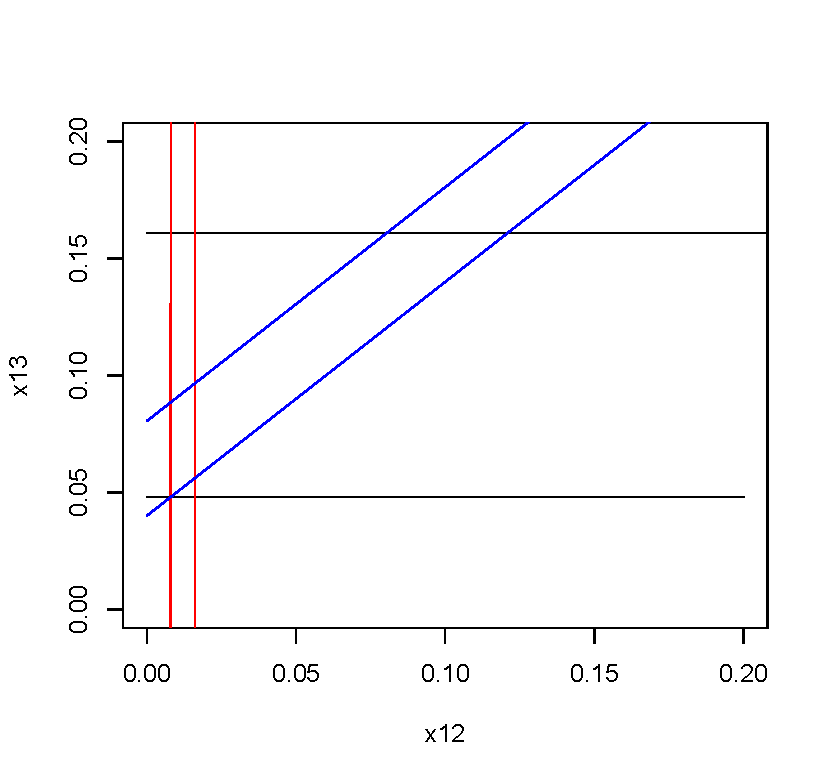
\includegraphics[width=4in]{3dxchoices.pdf}
\caption{The regions of $x-$space that give coexistence for the 3 possible species pairs. Species 1 and 2 can coexist between the red lines. Species 1 and 3 coexist between the black lines, while species 2 and 3 can coexist between the blue lines.}
\label{default}
\end{center}
\end{figure}
When species 3 dominates both species 1 and 2 (top left), it dominates the three species environment as expected, driving both other species to extinction. Similarly, when species 1 excludes each of the two less fecund species, it also dominates the three species case. However, when species 2 dominates both the more fecund species 1 and the faster growing species 3 in pairwise competition, in the right hand side region of Figure 1, where this occurs, there is an element of founder control. When species 3 excludes species 1 in pairwise competition, the outcome is driven by the initial populations, if species 2 is initially at a much lower population than species 3, species 3 will persist in monoculture, while if the initial population of species 2 is sufficiently high, it will exclude both the fecund species 1 and the fast growing species 3. Similarly, when species 1 excludes species 3, if the species 2 population in initially low, then species 1 will dominate the environment, while for higher initial populations species 2 dominates. When species 1 and 3 can coexist but are both excluded by species 2, in the three species case, it is necessary for species 2 to have a high initial population in order to persist, in which case it will exclude both other species. However, if it has a lower initial population, then it will be excluded and species 1 and species 3 will coexist together.

A similar pattern is observed when species 2 can coexist alongside one of the other species, yet excludes the third species. When species 2 and 3 can persist together, and species 2 excludes species 1, then founder control again occurs. If $n_2(0)$ is sufficiently high, species 1 will be driven to extinction and the species 2 and 3 coalition will persist, but if the initial population is too low, species 2 will be excluded, and the outcome of the model simulations is determined by the two species interactions between the fecund species 1 and the rapidly growing species 3. Similarly, when species 1 and 2 can coexist, and species 2 excludes species 3, a sufficiently low initial population will instead result in species 2 being excluded, and the outcome is determined by the interactions of species 1 and 3, while a high initial population will exclude species 3, allowing the species 1 and 2 coalition to thrive.

In all other cases, species 2 is excluded regardless of initial populations, and the behaviour of the model is determined by the two species analysis of species 1 and 3.

\subsection{Disturbance with equal effects on all species} \label{ss:homo}
When setting $I_i=I$ for all $i \in \{1,2,3\}$, such that disturbance effects all species equally, the response of the system to disturbance is determined by the non disturbance behaviour. We assume frequency is sufficiently high to not have a significant effect (see Chapter 2) and consider the impact of increasing disturbance intensity. If species 1 excludes both other species in a homogeneous environment, the only effect disturbance has is to accelerate this. When species 1 coexists with either species 2 or species 3 in the homogeneous environment, then as disturbance intensity increases, it will exclude the $K-$ competing species, although they will still coexist at low intensity. When either species 2 or species 3 exists in monoculture in a disturbance free environment, as intensity is increased they will coexist along side species 1. When intensity is increased further, species 1 will exclude the $K-$strategists. When species 2 and 3 coexist in the disturbance free case, intensity can cause different community structures. At low intensity, species 2 and 3 will continue to exclude species 1. As intensity increases, the generalist species 2 will exclude both the $K-$strategist species 3 and the $r-$strategist species 1. Increase intensity further, and species 1 and 2 will coexist while species 3 is excluded, while at very high intensities, species 1 will exclude both species 2 and 3.

\subsection{Adding a defence specialist}
In most cases, the generalist species 2 is outcompeted by the two specialists eroding some of its niche from either side. Does a specialisation in defence against disturbance allow species 2 to sustain itself alongside the growth and colonisation specialists? We set $I_1=I_3=yI_2$, and vary $y>1$ so examine the effects of defence specialism by species 2. We find that increasing the disturbance intensity will initially just repeat the anticipated behaviour when all 3 species suffer the same intensity.. For $y$ sufficiently close to 1 ($y=1.1$), this will continue and the `expected' behaviour will occur. However, for larger $y$ ($y=2,10$), as intensity is increased further, the advantage in disturbance survival for species 2 becomes the dominant force behind the dynamics, and both species 1 and 3 are excluded, with species 2 existing in monoculture. We conclude that resistance to disturbance mortality of the generalist cannot increase biodiversity along a fecundity-growth trade-off.

\subsection{Patchy disturbances; regions of the forest protected from disturbance}
When disturbance regimes do not differ, but one of the three species is absent initially from region $i$, allowing the region wide persistence of all three species, any $\alpha_{i,j},\alpha_{j,i}>0$ will result in region wide exclusion of one of the three species. We therefore focus on a region of trait space whereby any of the three species can persist at differing levels of intensity for high frequency disturbances. From \ref{ss:homo} we thus choose a region of $x-$space whereby the result in a homogeneous environment is that the $K-$strategist species 3 and the generalist species 2 coexist, while excluding species one. One such choice of parameters is given in Table~\ref{tab:paras}, which we use henceforth. Note that for these chosen parameters, species 2 will be excluded in the non disturbance case when it's initial population is too low. We select initial populations whereby species 2 has a sufficiently high population to persist in the environment ($n_{i,2}(0)=0.5N_i,n_{i,1}(0)=0.3N_i$). Then species 1 is present when disturbance frequency is high and for intensities $I\geq0.75$, which species 3 persists in the system for low intensities $I\leq 0.15$. Meanwhile, species 2 will persist for all intensities $I\leq 0.8$.
\begin{table}[htdp]
\begin{center}
\begin{tabular}{|c|c|} \hline
Parameter & Value\\ \hline
$s_1$&500\\
$s_2$&100\\
$s_3$&20\\
$x_{1,2}$&0.05\\
$x_{1,3}$&0.1\\
$N$&2000\\ \hline
\end{tabular}
\end{center}
\caption{Parameters used for examination of patchy disturbance}
\label{tab:paras}
\end{table}
We assume that Region 1 (size $N_1$) does not experience any disturbance (although simulations give qualitatively similar results providing the disturbance regime in this region is of sufficiently low intensity to allow the persistence of the least fecund species). For example, this may be a nature reserve where logging is prohibited, while the second region experiences disturbance via logging. Thus, when entirely unconnected to the second region, species 2 and 3 will persist. We then study the effects of varied intensities (homogeneous across all species) of disturbance in the second region for a fixed frequency ($T_D=5$), which also examining the impact of differing the size of the disturbed region in a total forest of fixed size $N=2000$, and the level of reproductive connectedness between the two patches. Note that $\alpha_{i,j}=N_j/N$ represents perfect mixing of the two populations, with entirely random seed allocation. Only disturbance intensities above $I_{2,k}=0.75$ (for $k=1,2,3$) are considered, to ensure that all three species are present when the regions are unconnected.

As connectedness of the two regions ($\alpha_{i,j}, i,j=1,2$) is increased, with seed dispersal or alternative processes such as human induced migration linking the two sites, it becomes possible for the regional processes allowing multi-species coexistence to inflate local biodiversity. As shown in Figure~\ref{fig:regions}, the migration of seeds creates coexistence of three species in the disturbed region 2, as the refuge region has much fewer gaps created. This makes it more difficult for the excluded, fecund, species to invade. In the disturbed region, however, there are a larger number of gaps are created when a disturbance occurs, thus increasing the probability of settlement by the poor coloniser (species 3), which would be excluded should there be no immigration from the refuge.

\begin{figure}[htbp]
\begin{center}
\includegraphics[width=4.5in]{RegionsPlot.pdf}
\caption{Restricted migration between a region without disturbance (region 1) and a region with high frequency, high intensity disturbances (region 2) can allow for three species coexistence at the local level. The disturbed region outside the refuge displays increased diversity when compared with regions that are not connected by seed dispersal, in which case the least fecund species would be excluded. Note that species richness within the refuge is not increased, despite the positive effect on regional richness.}
\label{fig:regions}
\end{center}
\end{figure}


\subsubsection{Effects of varied refuge patch size}
As the proportion of the forest protected from disturbance $N_1/N$ is varied, we find that the range of connectedness ($\alpha_{1,2}=\alpha_{2,1}=\alpha$, which is varied in increments of 0.05) for which all three species can persist at a given intensity is maximised at an intermediate value of $N_1/N$, as shown in Figure~\ref{fig:alpharange}. Only refuges below a certain proportion of the community can support all three species when there is mixing between the two regions. When the refuge becomes large, and the unprotected area small, the effect is to reduce the population of the fecund species 1. As this species requires the space creates by disturbance events to survive in the environment, the limited amount of space created by a disturbance, combined with the high mortality of species one in this part of the environment, results in the extinction of the most fecund species.

\begin{figure}[ht]
\label{fig:alpharange}
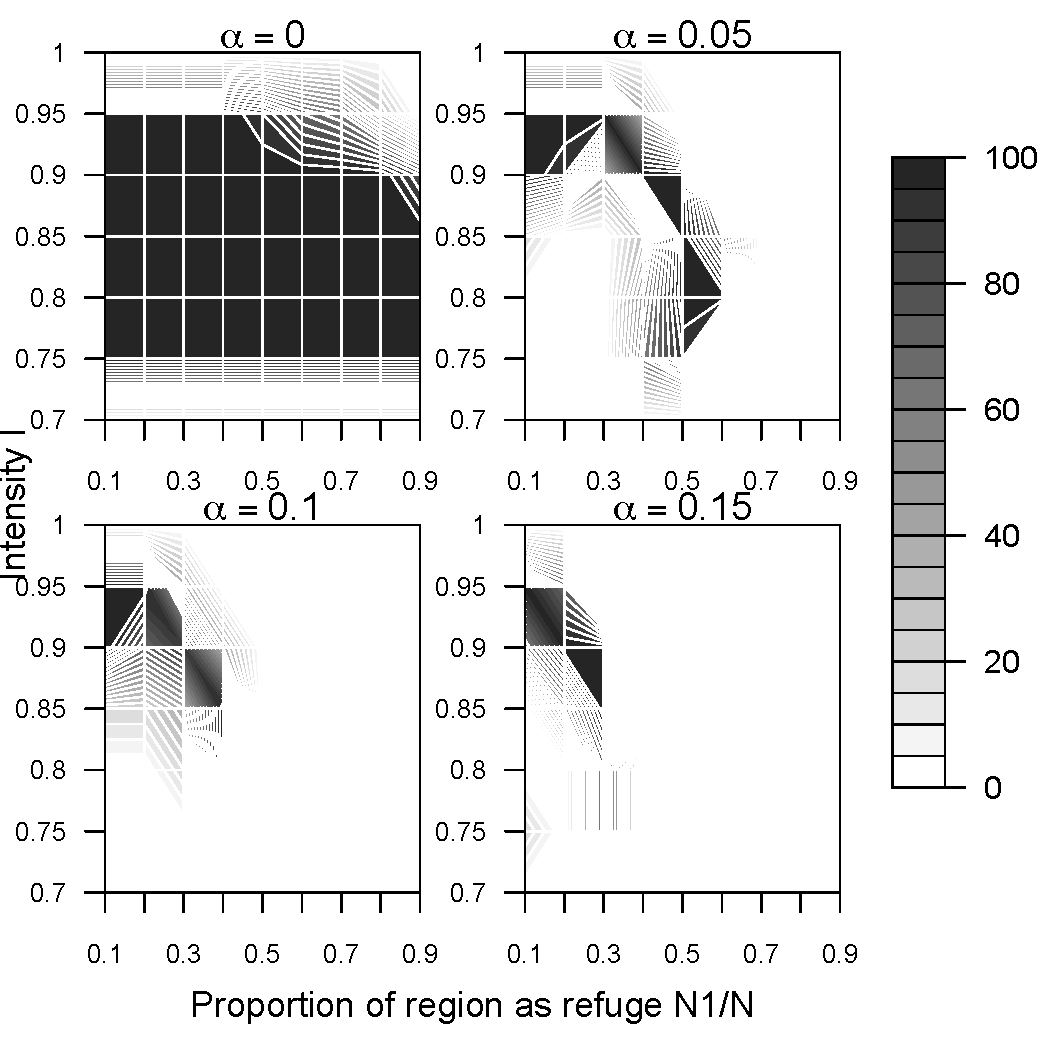
\includegraphics[width=4.5in]{refugesize.pdf}
\caption{The effects of varied refuge size of the likelihood of three species coexistence. Shaded areas represent the coexistence of all three species regionally after 50000 event time-steps. When $\alpha>0$, coexistence is only possible for relatively small refuges, while when the protected region is significantly larger than the disturbed area, coexistence is not possible for any non-zero level of cross-colonisation.}
\end{figure}

\section{Discussion}
Understanding the ways in species diversity is generated and supported is a crucial problem in ecology, with great relevance for conservation practices. The role of environmental variability, such as disturbance events, is an important area of consideration. This is becoming more crucial, as climate change is predicted to have dramatic impacts on the frequency and intensity of such events (REFS!!!!). Here, the possibility of multi-species ($n>2$) coexistence is examined in an environment defined by the disturbance regimes. Within this model framework, with species differing only along a fecundity-growth trade-off, it is only possible for more than two species to coexist if the environment has some spatial heterogeneity combined with the temporal heterogeneity of disturbance events. In this case, the existence of a protected region that does not experience disturbances that effect the neighbouring region (for example, a nature reserve where logging is prohibited, or a no-take zone alongside a heavily trawled region of ocean) can promote region wide coexistence of greater than two species. In addition, if limited dispersal occurs between the two regions, it is possible that the local species richness outside the protected region will also be increased, without observing a corresponding increase within the reserve. This may have important consequences for the placement and management of nature reserves, which often seek to cover environmental regions that support all species (e.g. \cite{margules1988selecting,scott2001nature}).

The coexistence of three species within this model framework appears to be more robust when the protected area, or refuge, is relatively small in comparison with the neighbouring environment. Small protected areas in large areas experiencing disturbance can enable the region-wide support of multiple species for much higher levels of dispersal between the disturbed and protected regions. This indicates that under some circumstances, where disturbance comes in the form of human pressure such as logging, it may be possible that careful management of the system would allow for a large area to be logged, while the region continues to support a large number of species.

However, it is only possible for two species to coexist when the environment is considered as a single patch, with no spatial heterogeneity, either with or without disturbance events. This result in the non-disturbance case, where the environment is both spatially and temporally homogeneous, lends support to previous predictions that coexistence is unlikely when species face a trade-off affecting per capita reproduction, such as the fecundity-growth trade-off considered here \cite{egas2004evolution}.
 However, these results appear to conflict with empirical data, where coexistence of generalists and specialists is common (e.g. \cite{morris1996coexistence} MORE REFS!). 
 
 Further, if all three species are present in a single, isolated patch at $t=0$, then the generalist species (here species 2) can only persist in the environment when the initial population is sufficiently high, in both environments with and without disturbance. This result is in contrast to those of both Marvier et al. \cite{marvier2004habitat} and Nagelkerke and Menken \cite{nagelkerke2013coexistence}, who find short term disturbances tend to favour generalist species. This difference may be caused by the assumption by Marvier et al. that species that spread tend to be generalists, while the model presented here assumes that the more fecund species is the most successful coloniser, and therefore is the species to benefit from the creation of a large number of empty sites. A second assumption here is that all species can survive in isolation across the entire disturbance gradient (providing $I_i<1$), and the niche segregation into fecundity specialist and light competition specialist is dependent on the specific species composition of the region. In contrast, both the model of Marvier et al. and that of Nagelkerke and Menken assume specialist species can only survive in certain habitat types, independent of the presence or absence of a competing species. The current model also predicts that allowing the generalist species an advantage in disturbance defence does not permit multi-species coexistence. This may be because an increase in fecundity and an increase in defence against disturbance effectively operate along the same environmental axis, both increasing fitness within a disturbance event.
 
 The results presented here emphasise that disturbance can be a key contributor to species richness, and that considering different factors that make up disturbance can be crucial in predicting how a community will respond to disturbance pressure (see also Chapter 2). Here, the effects of disturbance extent are examined, where a portion of the environment is protected, either naturally or by governmental policy, and demonstrate that this can help promote species richness at both a regional level and a local level. Perhaps counter-intuitively, it is possible to observe a increase in local diversity outside the refuge from disturbance, while no such increase is observed within the protected area. This suggests that  future empirical work should not only focus on events within the protected areas (e.g. \cite{pyvsek2002plant,kitchner1982predictors}), but must also consider the effects of introducing the reserve on neighbouring regions that remain unprotected.
 
